\documentclass[12pt]{article}
\usepackage{graphicx}
\usepackage{amsmath}
\usepackage{mathtools}
\let\vec\mathbf
\begin{document}
\begin{center}
\textbf\large{CHAPTER-7 \\ COORDINATE GEOMETRY}

\end{center}
\section*{Excercise 7.4}

\textbf{Q4.}The two opposite vertices of a square are $(–1, 2) \text{ and } (3, 2)$. Find the coordinates of the other two vertices.\\
\textbf{Solution :}

Given points $A =
\begin{pmatrix}
-1 \\
 2
\end{pmatrix},
C = 
\begin{pmatrix}
3\\
2
\end{pmatrix}$

Let $B = \begin{pmatrix}
x_{1}\\
y_{1}
\end{pmatrix} \text{ and }D = \begin{pmatrix}
x_{2}\\
y_{2}
\end{pmatrix} $
\begin{figure}[!h]
	\begin{center} 
	    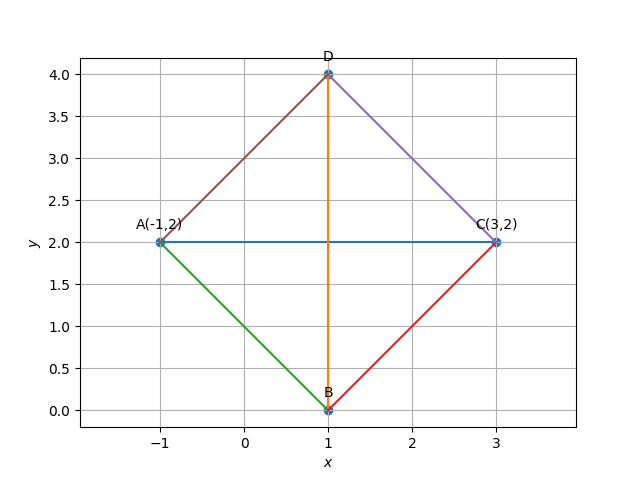
\includegraphics[width=\columnwidth]{./square}
	\end{center}
\caption{}
\label{fig:Fig1}
\end{figure}

Shifting point A to origin
$A' =
\begin{pmatrix}
0 \\
 0
\end{pmatrix}, 
B' = B-A = \begin{pmatrix}
x_{1}+1 \\
y_{1}-2 
\end{pmatrix}$

$C' = C-A = 
\begin{pmatrix}
4 \\
 0
\end{pmatrix} \text{ and } 
D' = D-A = 
\begin{pmatrix}
x_{2}+1 \\
y{2}-2
\end{pmatrix}$

\begin{figure}[!h]
	\begin{center} 
	    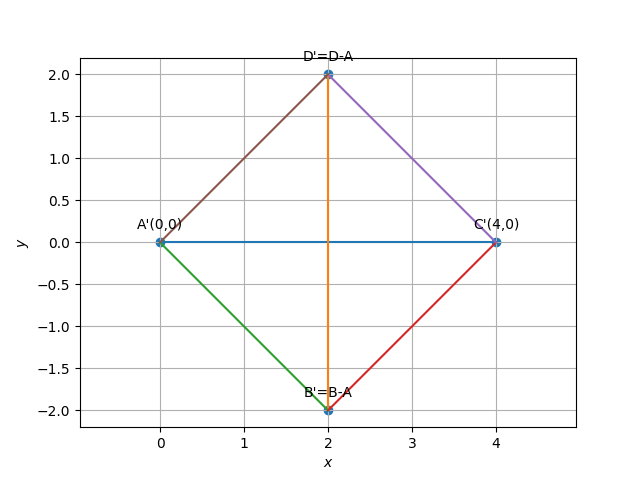
\includegraphics[width=\columnwidth]{./square1}
	\end{center}
\caption{}
\label{fig:Fig1}
\end{figure}


Now caculating the angle the $\vec{AB}$ makes with the x-axis.

Let $\vec{AB}$ makes an angle $\theta$ with the x-axis and we know $\angle C'A'B' = 45^{\circ}$

Angle made by $\vec{AC} = \theta + 45 $ on the x-axis
\begin{align*}
tan(\theta + 45) &= \frac{0-0}{4-0}\\
\theta &= -45^{\circ}
\end{align*}

We know the rotation matrix is given as
$P =
\begin{pmatrix}
cos\theta & -sin\theta \\
sin\theta & cos\theta
\end{pmatrix}
$

Now the transformed coordinates are 
\begin{align*}
C" = P(C-A) =
\begin{pmatrix}
\frac{1}{\sqrt{2}} & \frac{1}{\sqrt{2}} \\
-\frac{1}{\sqrt{2}} & \frac{1}{\sqrt{2}}
\end{pmatrix}
\begin{pmatrix}
4 \\
0
\end{pmatrix} = 
\begin{pmatrix}
\frac{4}{\sqrt{2}} \\
-\frac{4}{\sqrt{2}}
\end{pmatrix}
\end{align*}
\begin{align*}
B" = \begin{pmatrix}
 0\\
 -\frac{4}{\sqrt{2}}
\end{pmatrix},
D" = \begin{pmatrix}
 \frac{4}{\sqrt{2}}\\
 0
\end{pmatrix} \text{ and }
A" =
\begin{pmatrix}
0 \\
 0
\end{pmatrix}
\end{align*}

\begin{figure}[!h]
	\begin{center} 
	    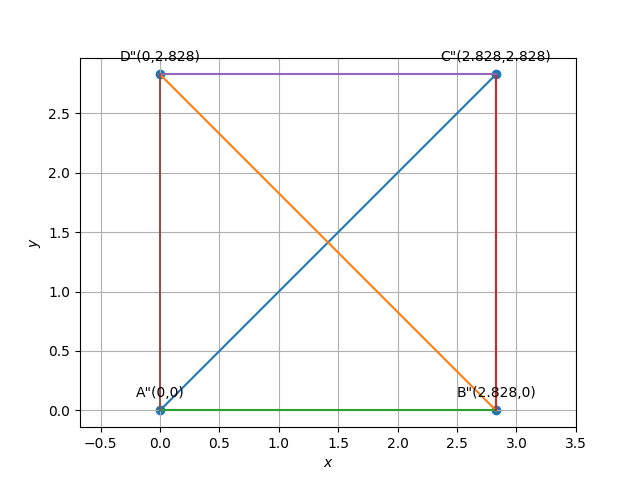
\includegraphics[width=\columnwidth]{./square2}
	\end{center}
\caption{}
\label{fig:Fig1}
\end{figure}

Again tranforming the coordinates back to the original axis.

We know for anti-clockwise direction the rotation matrix is given as
$$P =
\begin{pmatrix}
cos\theta & sin\theta \\
-sin\theta & cos\theta
\end{pmatrix}
$$

So now the transformed coordinates B and D will be
\begin{align*}
B' &= PB" = \begin{pmatrix}
\frac{1}{\sqrt{2}} & -\frac{1}{\sqrt{2}} \\
\frac{1}{\sqrt{2}} & \frac{1}{\sqrt{2}}
\end{pmatrix}
\begin{pmatrix}
 0\\
 -\frac{4}{\sqrt{2}}
\end{pmatrix} = 
\begin{pmatrix}
2 \\
-2
\end{pmatrix}\\
D' &= PD" = \begin{pmatrix}
\frac{1}{\sqrt{2}} & -\frac{1}{\sqrt{2}} \\
\frac{1}{\sqrt{2}} & \frac{1}{\sqrt{2}}
\end{pmatrix}
\begin{pmatrix}
 \frac{4}{\sqrt{2}}\\
 0
\end{pmatrix} = 
\begin{pmatrix}
2 \\
2
\end{pmatrix}\\
\end{align*}

\begin{figure}[!h]
	\begin{center} 
	    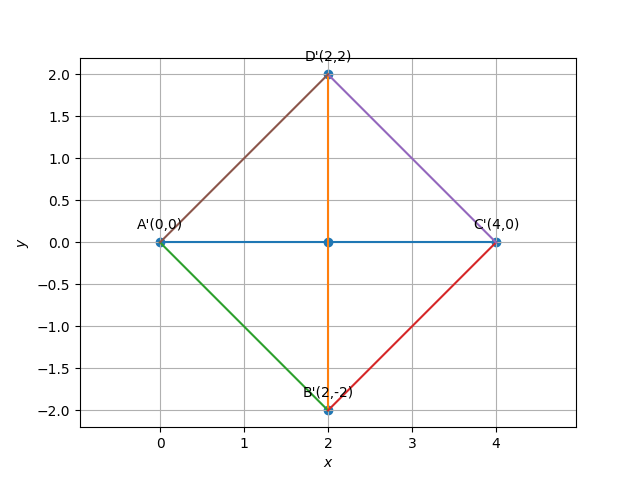
\includegraphics[width=\columnwidth]{./square3}
	\end{center}
\caption{}
\label{fig:Fig1}
\end{figure}

Again transforming the axis back to the original
\begin{align*}
B &= B'+A = \begin{pmatrix}
2 \\
-2
\end{pmatrix}+\begin{pmatrix}
-1 \\
2
\end{pmatrix} = 
\begin{pmatrix}
1 \\
0
\end{pmatrix}\\
D &= D'+A = \begin{pmatrix}
2 \\
2
\end{pmatrix}+\begin{pmatrix}
-1 \\
2
\end{pmatrix} = 
\begin{pmatrix}
1 \\
4
\end{pmatrix}
\end{align*}

Hence, the other two vertices are $B(1,0) \text{ and } D(1,4)$   

\begin{figure}[!h]
	\begin{center} 
	    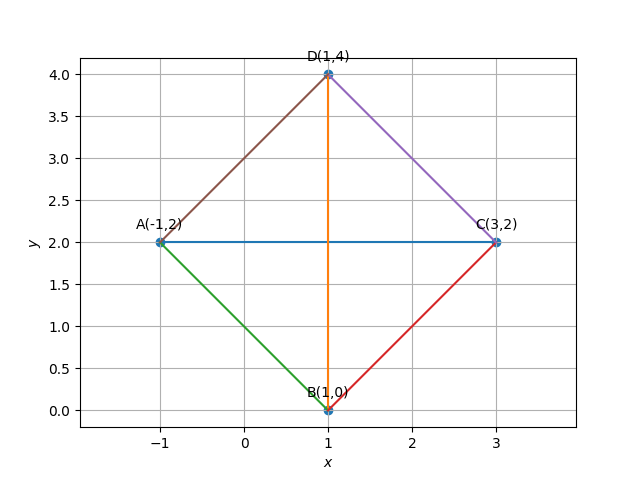
\includegraphics[width=\columnwidth]{./square4}
	\end{center}
\caption{}
\label{fig:Fig1}
\end{figure}





\end{document}